%%%%%%%%%%%%%%%%%%%%%%%%%%%%%%%%%%%%%%%%%
% NIWeek 2014 Poster by T. Reveyrand
% www.microwave.fr
% http://www.microwave.fr/LaTeX.html
% ---------------------------------------
% 
% Original template created by:
% Brian Amberg (baposter@brian-amberg.de)
%
% This template has been downloaded from:
% http://www.LaTeXTemplates.com
%
% License:
% CC BY-NC-SA 3.0 (http://creativecommons.org/licenses/by-nc-sa/3.0/)
%
%%%%%%%%%%%%%%%%%%%%%%%%%%%%%%%%%%%%%%%%%

%----------------------------------------------------------------------------------------
%	PACKAGES AND OTHER DOCUMENT CONFIGURATIONS
%----------------------------------------------------------------------------------------

\documentclass[ansiepaper,portrait]{baposter}

\usepackage[font=small,labelfont=bf]{caption} % Required for specifying captions to tables and figures
\usepackage{booktabs} % Horizontal rules in tables
\usepackage{relsize} % Used for making text smaller in some places

\usepackage{amsmath,amsfonts,amssymb,amsthm} % Math packages
\usepackage{eqparbox}

\usepackage{textcomp}
\usepackage{multicol}
\usepackage{wrapfig} % Allows wrapping text around tables and figures

\graphicspath{{figures/}} % Directory in which figures are stored

 %\definecolor{bordercol}{RGB}{40,40,40} % Border color of content boxes
 \definecolor{bordercol}{RGB}{186,215,230} % Border color of content boxes

 \definecolor{headercol1}{RGB}{0,102,51} % Background color for the header in the content boxes (left side)
\definecolor{headercol2}{RGB}{0,102,51} 
% \definecolor{headercol2}{RGB}{120,120,120} % Background color for the header in the content boxes (right side)
 \definecolor{headerfontcol}{RGB}{256,256,256} % Text color for the header text in the content boxes
 %\definecolor{boxcolor}{RGB}{210,235,250} % Background color for the content in the content boxes
\definecolor{boxcolor}{RGB}{250,250,250}

\renewcommand\refname{\vskip -1cm}

\begin{document}
\background{}

\begin{poster}{
grid=false,
borderColor=bordercol, % Border color of content boxes
headerColorOne=headercol1, % Background color for the header in the content boxes (left side)
headerColorTwo=headercol2, % Background color for the header in the content boxes (right side)
headerFontColor=headerfontcol, % Text color for the header text in the content boxes
boxColorOne=boxcolor, % Background color for the content in the content boxes
headershape=roundedright, % Specify the rounded corner in the content box headers
headerfont=\Large\sf\bf, % Font modifiers for the text in the content box headers
textborder=rectangle,
background=user,
headerborder=open, % Change to closed for a line under the content box headers
boxshade=plain
}
{
\includegraphics[scale=0.10]{logo_davidson.png}}
%
%----------------------------------------------------------------------------------------
%	TITLE AND AUTHOR NAME
%----------------------------------------------------------------------------------------
%
{ \bf  \huge {A Streamlined Python Framework for AT-TPC Data Analysis} }
%\Large \it A} % Poster title
{\vspace{0.3em} \smaller Jack Taylor and Dr. Michelle Kuchera \\  % Authors
  
\smaller \it {Department of Physics, Davidson College, Davidson, NC 28035}} % Author email addresses
{
\includegraphics[scale=0.3]{nscl_logo.png}} % University/lab logo

%----------------------------------------------------------------------------------------
%	ABSTRACT
%----------------------------------------------------------------------------------------
\headerbox{Abstract}{name=abstract,column=0,row=0, span=3}{
\small{Data-analysis software for the Active-Target Time Projection Chamber (AT-TPC) at the National Superconducting Cyclotron Laboratory (NSCL) was documented and used to analyze unbound states in Argon-40 ($^{40}$Ar). NSCL is a national user facility funded by the National Science Foundation that provides rare isotope beams to researchers around the world to study cutting-edge nuclear physics phenomena. Rare isotope beams are produced, accelerated, and delivered to various experimental setups, each with their own physics motivations. One such setup is the AT-TPC, a gas-filled detector that acts as both the detector and target for high-efficiency detection of low-intensity, exotic nuclear reactions. The pytpc framework is a Python package for analyzing AT-TPC data and was developed for the analysis of $^{46}$Ar(p, p) data. The existing software was used to analyze data produced by the $^{40}$Ar(p, p) experiment that ran in August, 2015. Usage of the package was documented in an analysis manual both to improve analysis steps and aid in the work of future AT-TPC users. Software features and analysis methods in the pytpc framework will be presented along with the $^{40}$Ar results.}
}
%----------------------------------------------------------------------------------------
%	THE AT-TPC
%----------------------------------------------------------------------------------------
\headerbox{The Active-Target Time Projection Chamber}{name=attpc,column=1,row=1,span=2,below=abstract}
{\small{The AT-TPC is a gas-filled detector that acts as both the detector and target for high-efficiency detection of low-intensity, exotic nuclear reactions. Because the gas target also acts as the detector, the AT-TPC is highly efficient, providing nearly ${4\pi}$ angular coverage. The AT-TPC operates inside a nearly 2 Tesla solenoidal magnetic field. Reactions can be measured over a wide range of energies as the beam loses energy in the gas \cite{ATTPC-NIM}.
In order to obtain this ${4\pi}$ coverage with high resolution, a highly segmented pad plane captures the detector signal. There are 10240 pads in the pad plane which produces on the order of 10MB of data per event.}

\begin{center}
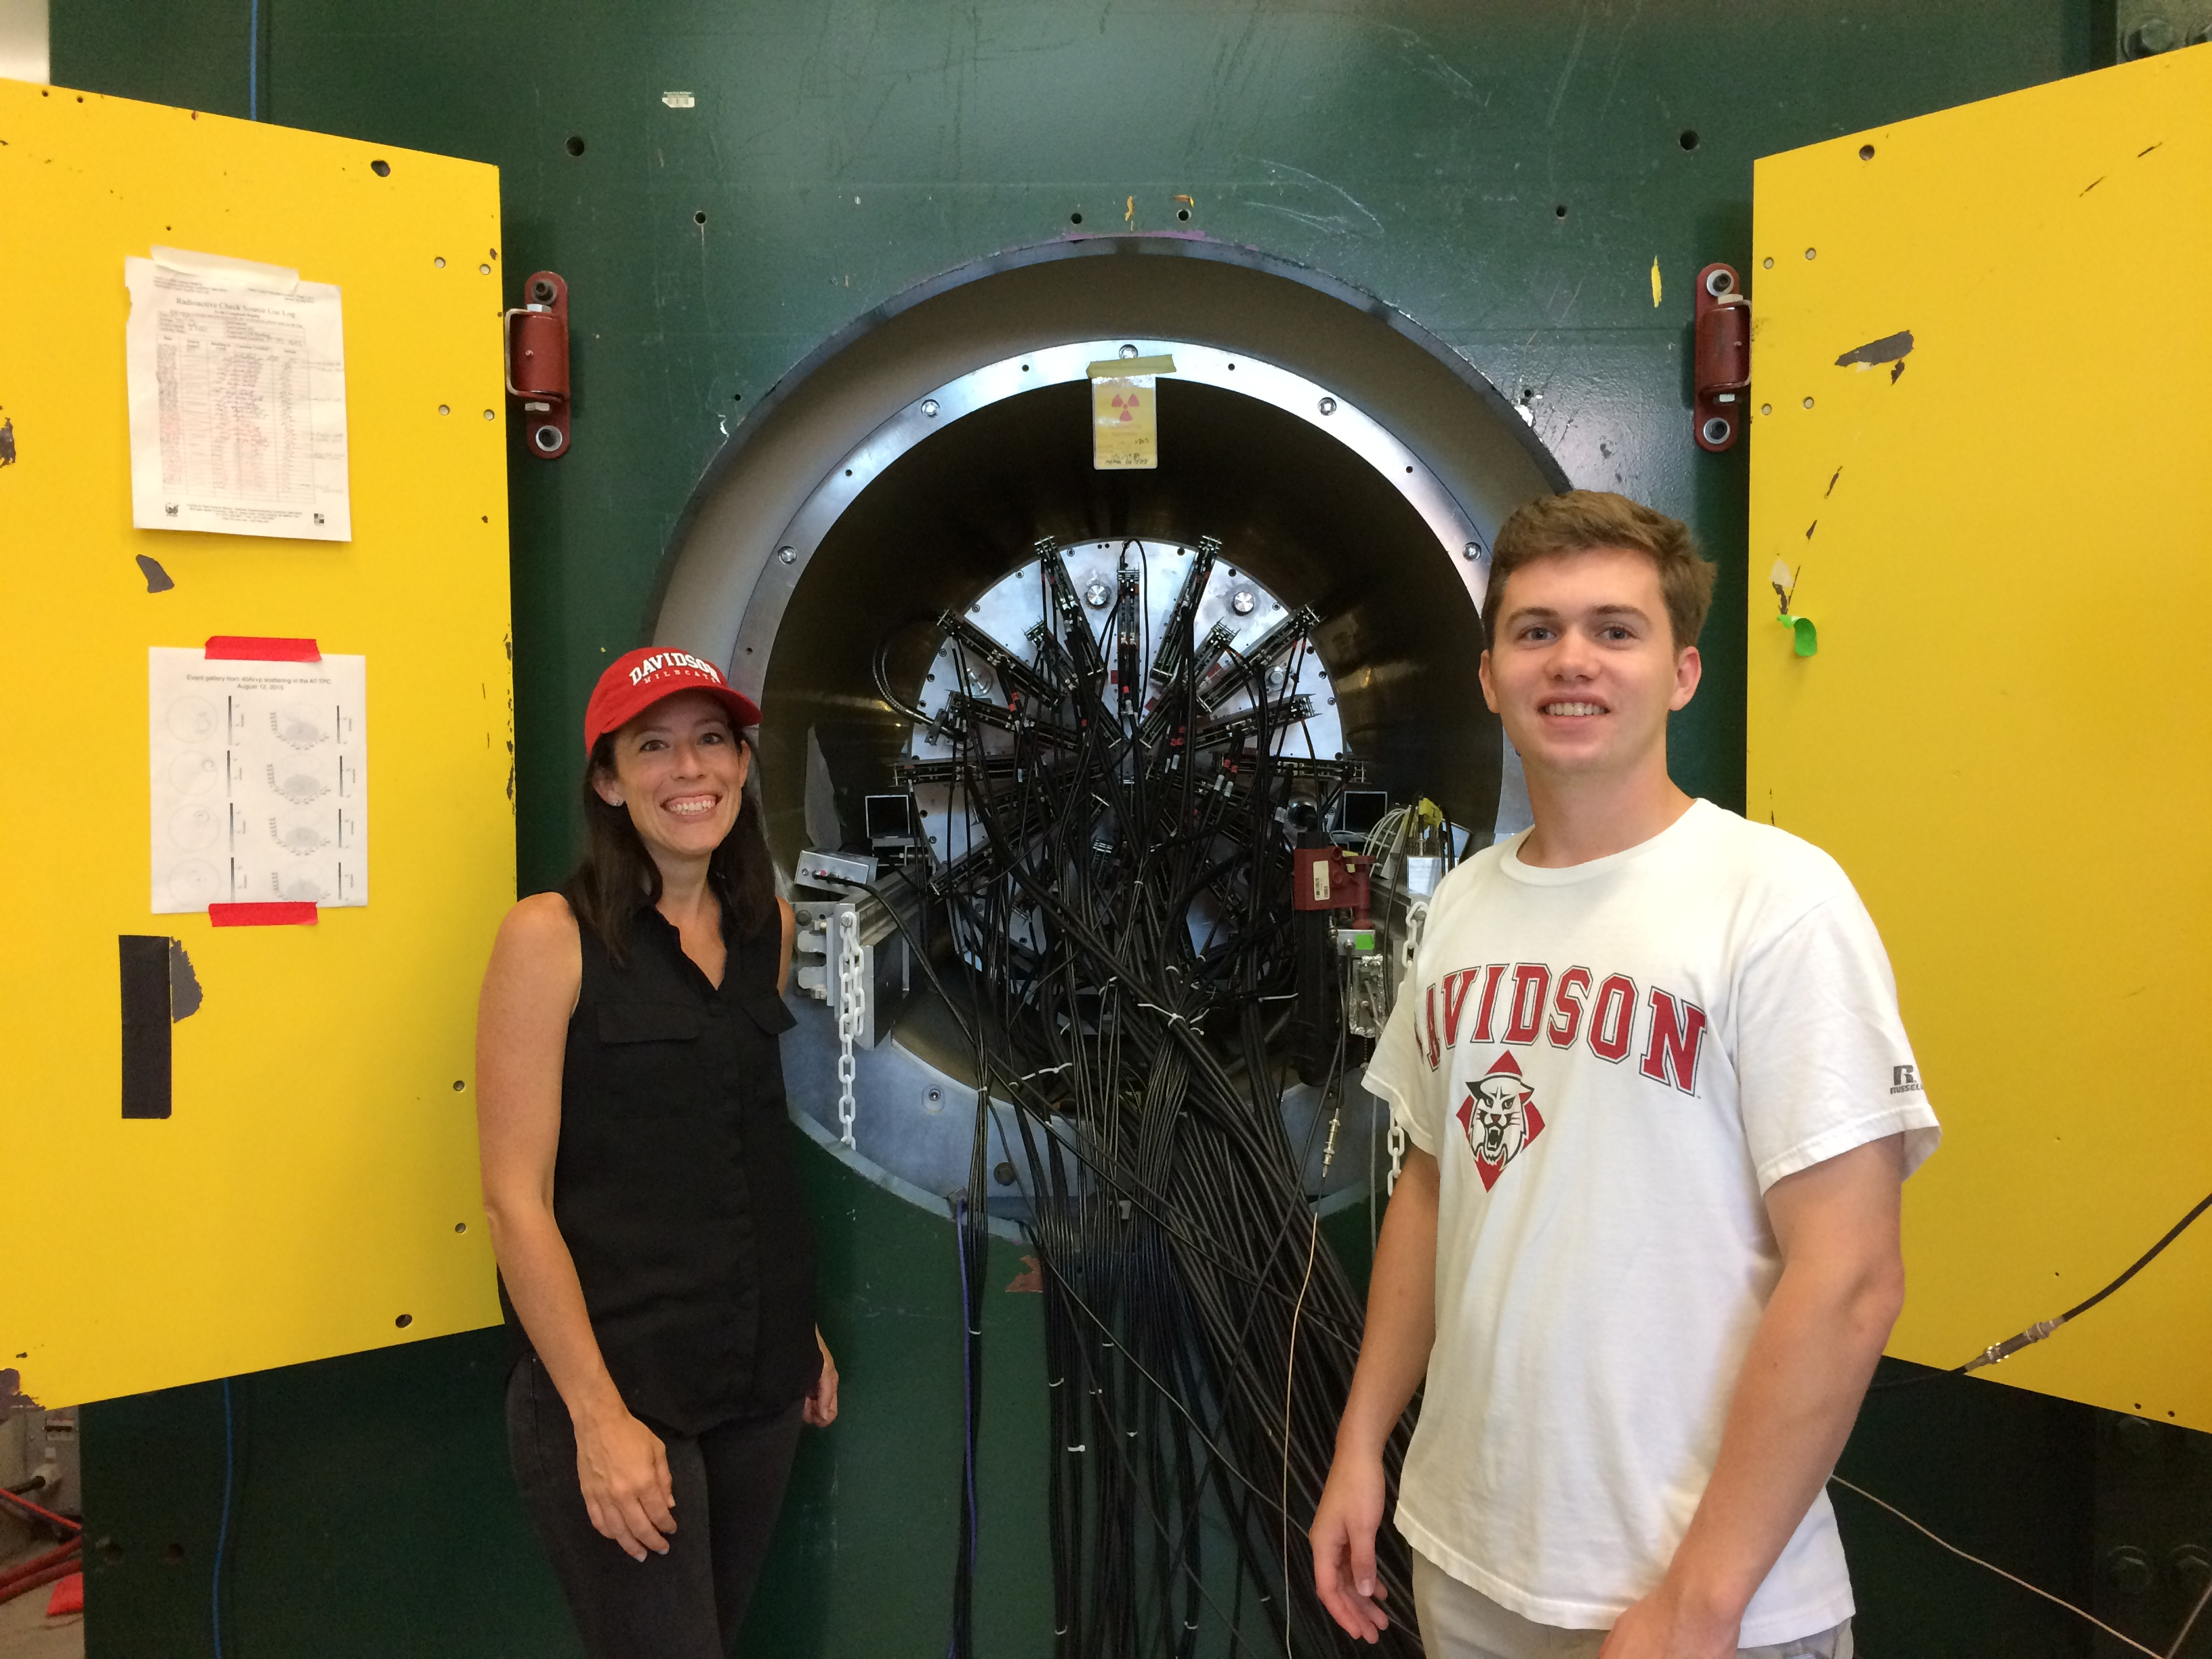
\includegraphics [height=30mm]{michigan_trip.jpg} 
\hspace{0.2cm}
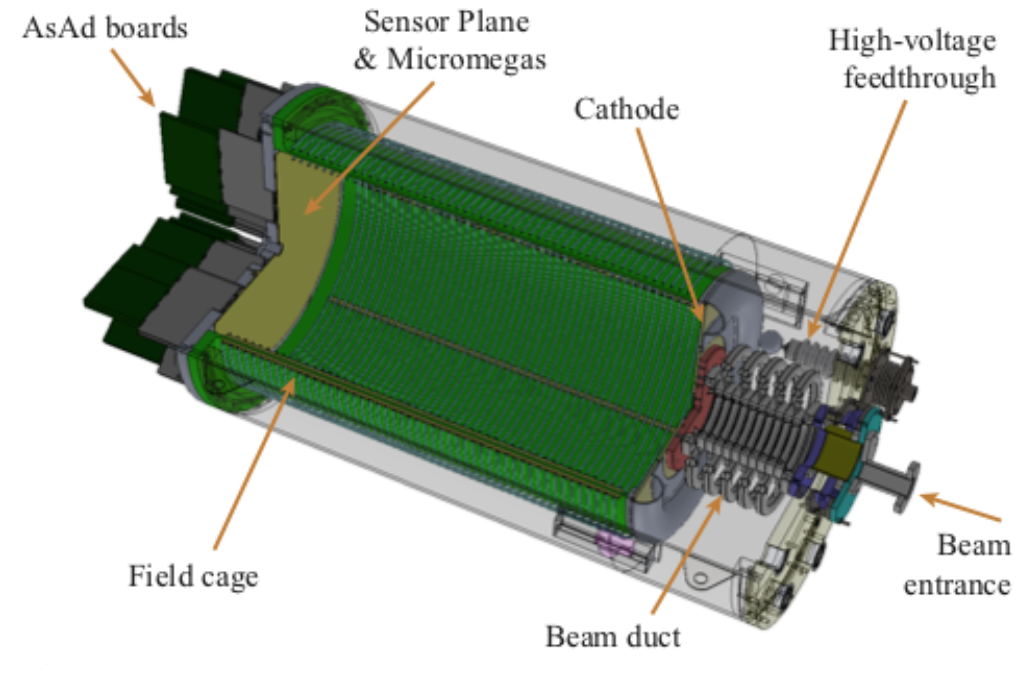
\includegraphics [height=30mm] {attpc.png}
\end{center}

\small{\textbf{Figure 2.} This is a schematic of the AT-TPC. The rare isotope beam enters the the detector on the right-hand side and moves left towards the sensor plane \cite{Bradt-thesis}.}


\small{\textbf{Figure 3.} Right, This is a photograph of the backside of the AT-TPC lkdda.}

}
%----------------------------------------------------------------------------------------
%	Motivation
%----------------------------------------------------------------------------------------
\headerbox{Motivation}
{name=motivation,column=0,row=1,below=abstract}
{\small{The study of rare isotopes has applications ranging far beyond the quest for universal discovery, from national security to medicine. Experimental endeavors using low-intensity beams of radioactive ions introduce unique challenges in experimental design and analysis. Rare isotope beams typically have low intensity, leading to fewer reactions and events, thus requiring a detector with high efficiency. The AT-TPC was conceived, designed, and built for improved data acquisition for rare isotope experiments. 
This project involved creating an analysis manual and framework documentation to streamline the analysis process for future users and increase the accessibility of the software as well as analyzing data from the $^{40}$Ar(p,p) reaction.}

\begin{center}
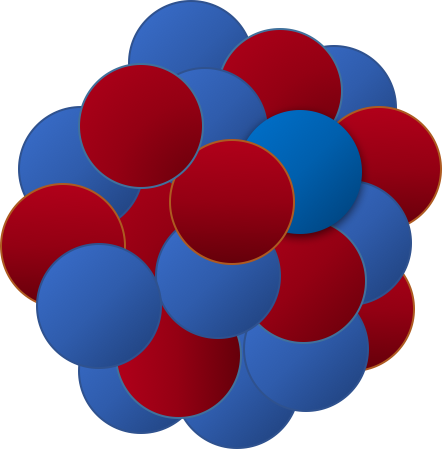
\includegraphics[width=25mm]{ar40_nucleus.png}
\end{center}

\small{\textbf{Figure 1.} This is a diagram of a $^{40}$Ar nucleus.}
}
%----------------------------------------------------------------------------------------
%	40AR ANALYSIS
%----------------------------------------------------------------------------------------
\headerbox{Analysis of the $^{40}$Ar Beam Experiment Data}{name=analysis,span=2,column=1,row=1, below=attpc}
{\small{The analysis code, originally written for a $^{46}$Ar data, was applied to data from the $^{40}$Ar(p, p) experiment that ran at the NSCL in August,  2015.}
\small{The Monte Carlo fit results provide the vertex position of a reaction in the detector chamber. The energy of the beam particle at this location can be found by calculating the energy lost by the particle to the gas target that fills the chamber.}

\begin{center}
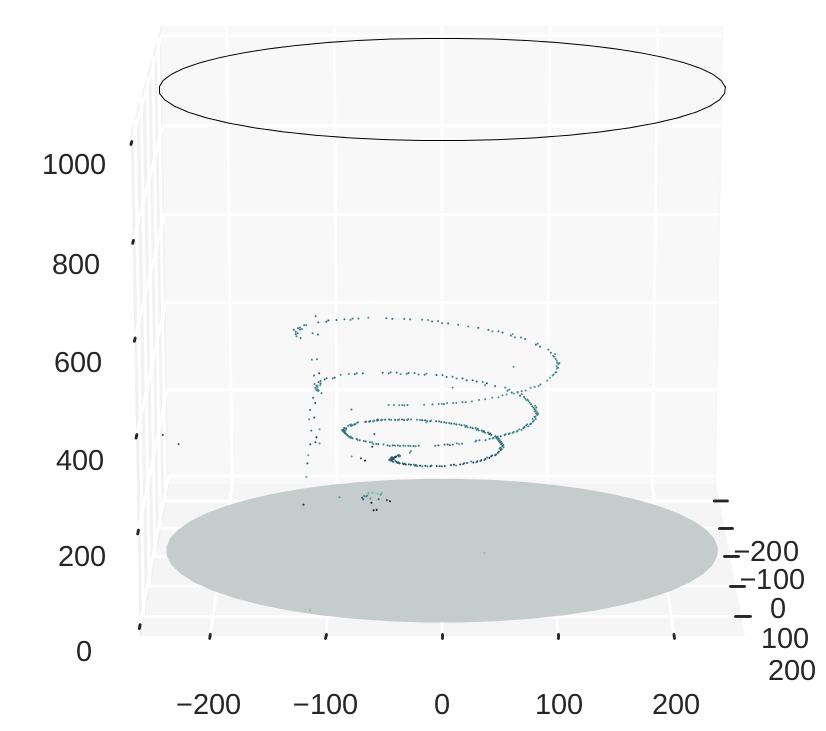
\includegraphics[height=30mm]{chamber_plot.png}
\hspace{.5cm}
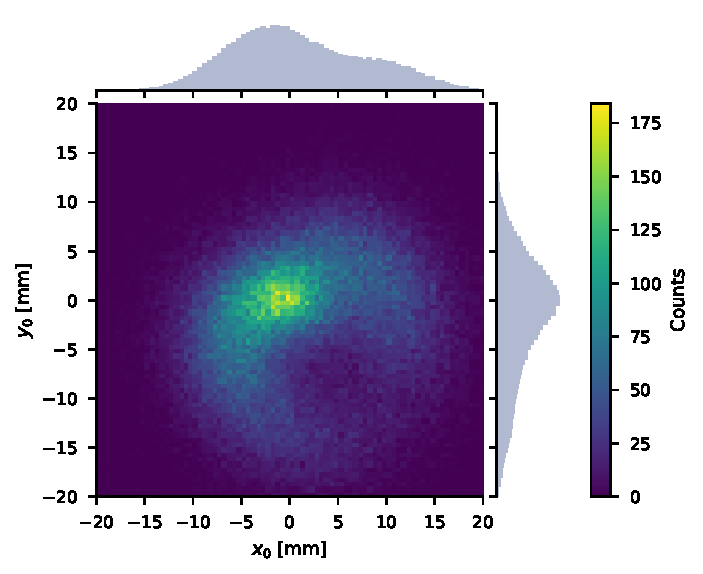
\includegraphics [height=30mm, width=43mm] {vertex_pos_distrib.pdf}
\hspace{.5cm}
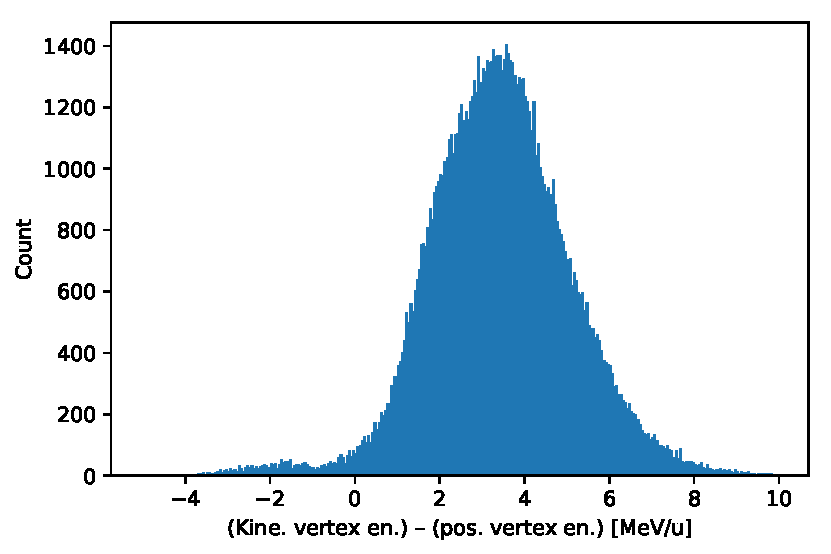
\includegraphics [height=30mm, width=43mm] {vertex_en_error.pdf}
\end{center}

\small{\textbf{Figure 2.} This is an example of a proton event rendered in the pytpc framework.}

\small{\textbf{Figure 4.} Left, distribution of vertex positions in the plane transverse to the detector.}

\small{\textbf{Figure 5.} Right, difference between the vertex energy as calculated from kinematics and vertex position. The trend of the count away from 0 on the x-axis is indicative of a problem with the vertex energy calculated from kinematics.}

\begin{center}
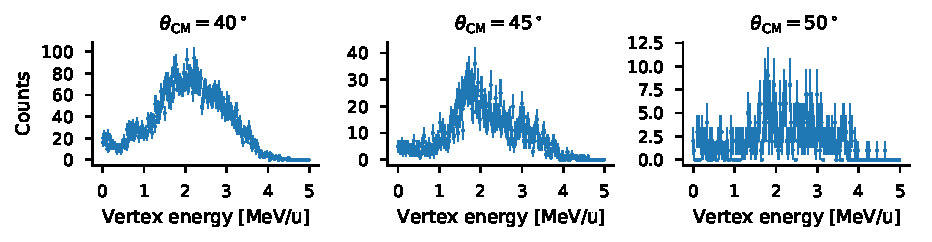
\includegraphics [width=100mm] {angular_excitation_hists_POSTER.pdf}
\end{center}
\small{\textbf{Figure 6.} Unnormalized excitations functions as a function of the $^{40}$Ar vertex energy in the laboratory frame shown for multiple center-of-mass scattering angles ($\theta_{cm}$).}
}

%----------------------------------------------------------------------------------------
%	CONCLUSION - FUTURE
%----------------------------------------------------------------------------------------
\headerbox{Conclusion and Future Work}{name=conclusion,column=1,below=analysis,span=2}
{\small{ By analyzing the data from the $^{40}$Ar experiment I gained firsthand experience with the software I was documenting, examined data that was previously unused, and tested the adaptability of the software. The analysis manual for the pytpc framework will help experimentalists from around the world apply pytpc data produced by their own AT-TPC experiments.
I will be continuing my work with AT-TPC data and the analysis process this semester in a more research-focused capacity. My current research will explore and apply machine learning methods to the issue of event classification for AT-TPC data. Ideally this will increase statistics and reduce both error and computational time. }
}
%----------------------------------------------------------------------------------------
%	REFERENCES
%----------------------------------------------------------------------------------------
\headerbox{References}{name=references,column=0,above=bottom,span=1}{
\footnotesize{\bibliographystyle{unsrt}
\hspace{.05cm}
\itemsep-0.5em
\bibliography{bibliography.bib}}
}
%----------------------------------------------------------------------------------------
%	PYTPC
%----------------------------------------------------------------------------------------
\headerbox{The pytpc Framework}{name=pytpc,column=0,row=2, above=references, below=motivation}
{\small{The pytpc framework is a Python package for analyzing AT-TPC data. The package provides functions for reconstructing, cleaning, and fitting particle tracks produced by beam experiments run on the AT-TPC. Analysis of AT-TPC data is a multi-step process:

\begin{enumerate}\itemsep-0.2em
\item Baseline Correction for Electronics Signals
\item Track Reconstruction
\item Removal of Noise Using a Hough Transform
\item Modeling and Fitting Tracks with a Monte Carlo Optimizer
\end{enumerate}

\begin{center}
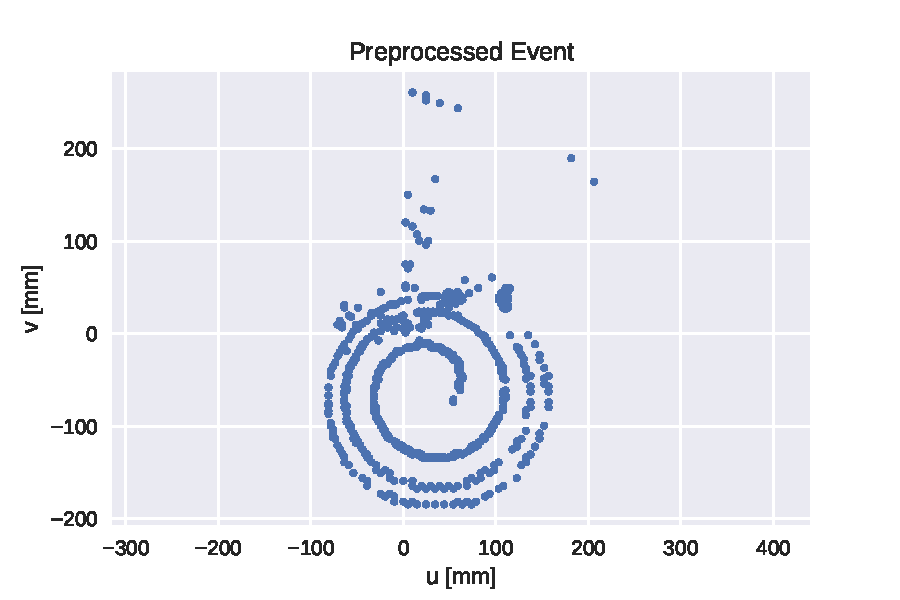
\includegraphics [width=21mm] {preprocess_evt.pdf}
\hspace{.3cm}
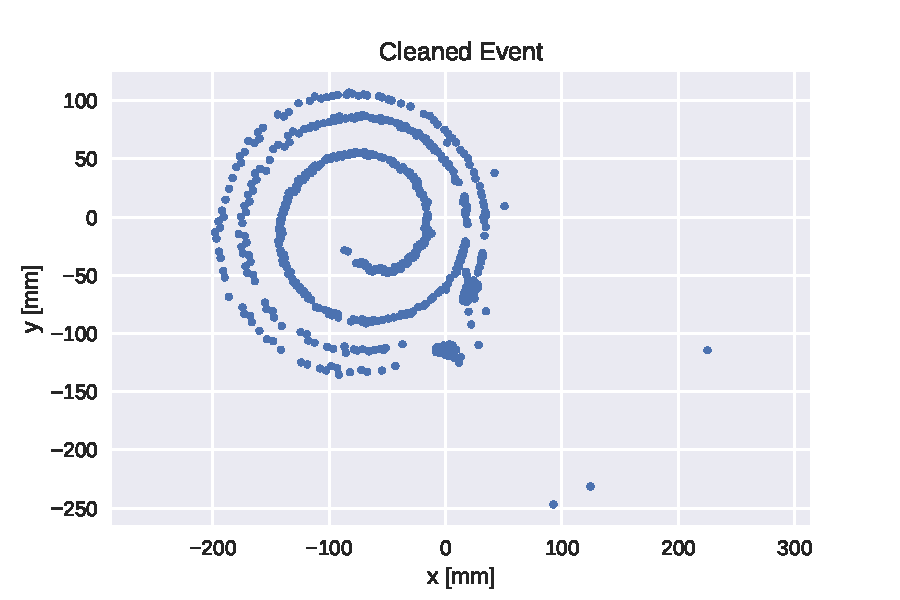
\includegraphics [width=21mm] {clean_evt.pdf}
\hspace{.3cm}
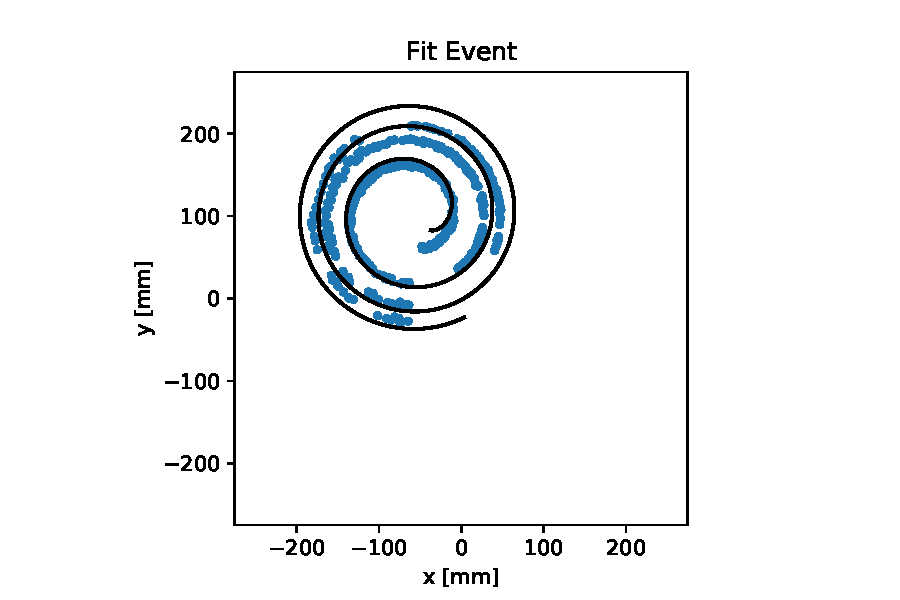
\includegraphics [width=21mm] {fit_evt.pdf}
\end{center}
\textbf{Figure 3.} From left to right,  Here are examples of a preprocessed event, an event after the Hough Transform cleaning, and a Monte Carlo fit event.}

%\begin{center}
%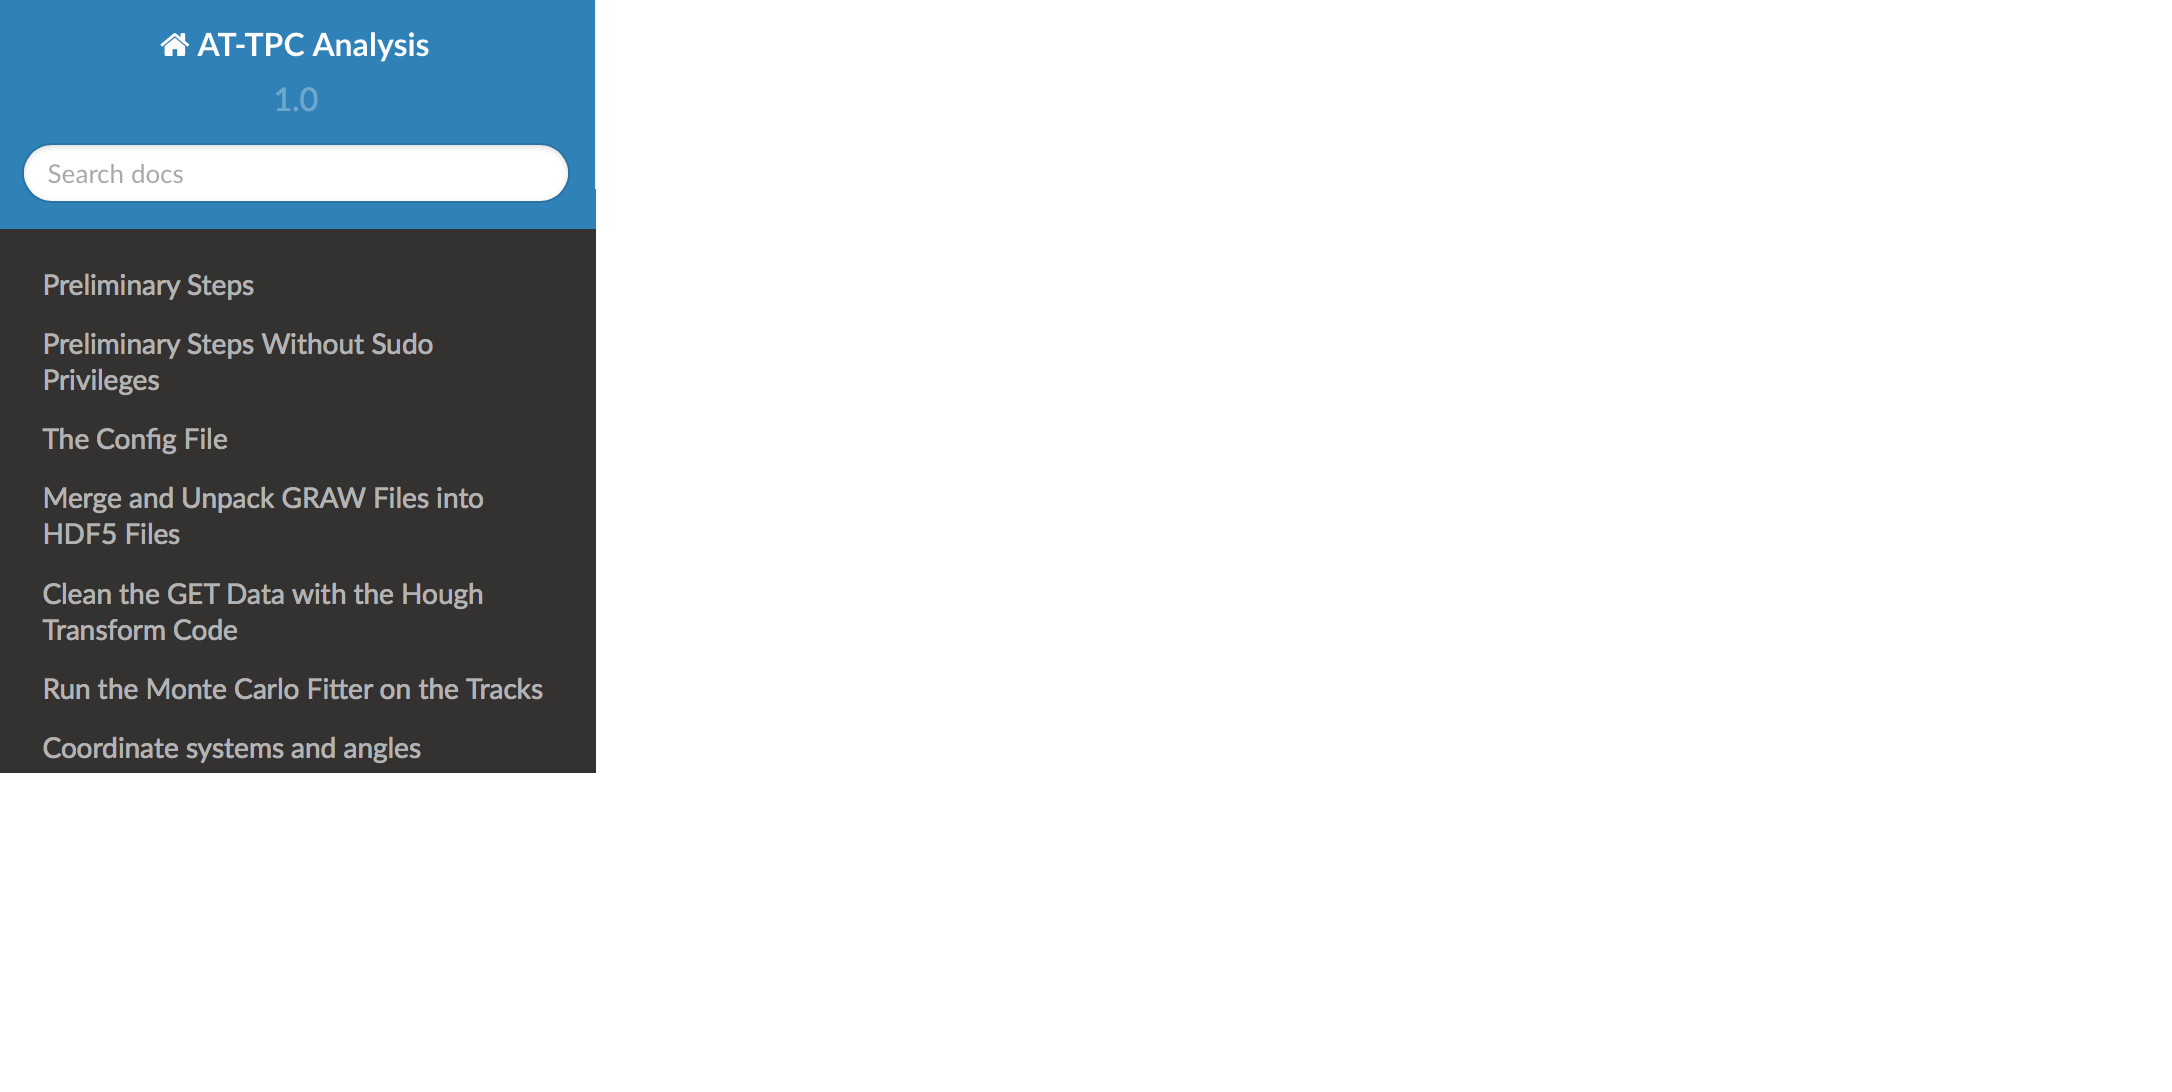
\includegraphics [height=40mm] {documentation.png}
%\end{center}

} 


\end{poster}
\end{document}
